% -*- coding: utf-8 -*-
\newpage
\section{{\selectlanguage{hebrew}חלום יעקב} (Jacob's Dream)}

\begin{flushright}
\textit{the author writes here not as a scientist,}
\end{flushright}

As a theoretical chemist and an \emph{enthusiast} of art, i've always found it
a little unsatisfying that most of the visual representations of Jacob's Ladder
in \gls{DFT} are, let's say, not exactly the most beautiful images ever created
(no offence to their authors!). We might be missing a chance to reimagine it,
to create a representation that captures not only the technical content but also
the metaphorical and symbolic richness behind it.

On one hand, i get it. Not everyone wants their science mixed with metaphors,
religion, or artistic flourishes. Some just want equations, data, numbers
and that's completely fine. It's also true that many of us are cautious
about including anything that might be interpreted as pushing a particular faith
or worldview into scientific spaces.

But even so... we're missing something! We're missing the opportunity to make
something ---something visual, symbolic, maybe even a bit poetic and just for
fun, as a side project during free time--- that reflects the deeper meaning of
this metaphor.

The ``Jacob’s Ladder'' in \gls{DFT} is, of course, a reference to the biblical one.
According to the Book of Genesis, the patriarch Jacob had a dream while resting
for the night, using a stone as his pillow. In that dream, he saw a ladder
reaching from the earth up to the heavens, with angels ascending and descending
upon it.

In the context of \gls{DFT}, the ladder becomes a metaphor: we begin with
\gls{HF}, and we aim for the heaven, that is, for chemical accuracy. We climb
rung by rung, from \gls{LDA} to \gls{GGA}, and onward to meta-GGAs, hybrids,
double hybrids... each rung represents a systematic improvement, a deliberate
step upward in complexity and (ideally) accuracy.

Just like in the biblical interpretations, we don't take a single miraculous
leap from earth to sky. Instead, we follow a structured path, becuase...  if
angels can fly, why would they need a ladder?, maybe because the ladder wasn't
built for them. It was built for us. We don't need wings. We don't need to
mimic the angels. We just need a clear and methodical way to ascend. Not by
miracle, but by method.

\newpage
Perdew himself offered a beautiful interpretation of his metaphor
in~\cite{Perdew2013}. In his words, the angels on the ladder are the users:
researchers who choose the rung that best suits their needs, depending on
the balance they seek between accuracy and computational cost.

Personally, I like to think of the angels in two ways: some go up, carrying the
prayers ---input files, basis sets, SCF settings--- of the users; others come
down bearing blessings converged energies and properties. Just like a biblical
interpretation, where the angels ascending represent the prayers and the ones
descending are the messengers of God (\emph{intentional redundancy}) with the divine
blessing for those who pray.

Note that we can't know which angel is in front of other, just by the
knowledge of the rung, we need to know the direction of the angel; as well
as in the rungs of \gls{DFT} Jacob's Ladder, some times our goal is
to ascend in the ladder, seeking more accuracy, and sometimes we need to
descend, looking for a faster calculation.

Our feet stay grounded in practical considerations, but our eyes are fixed on
the sky. It's not blind faith, it's a slow, structured journey up the ladder.

\begin{figure}
  \centering
  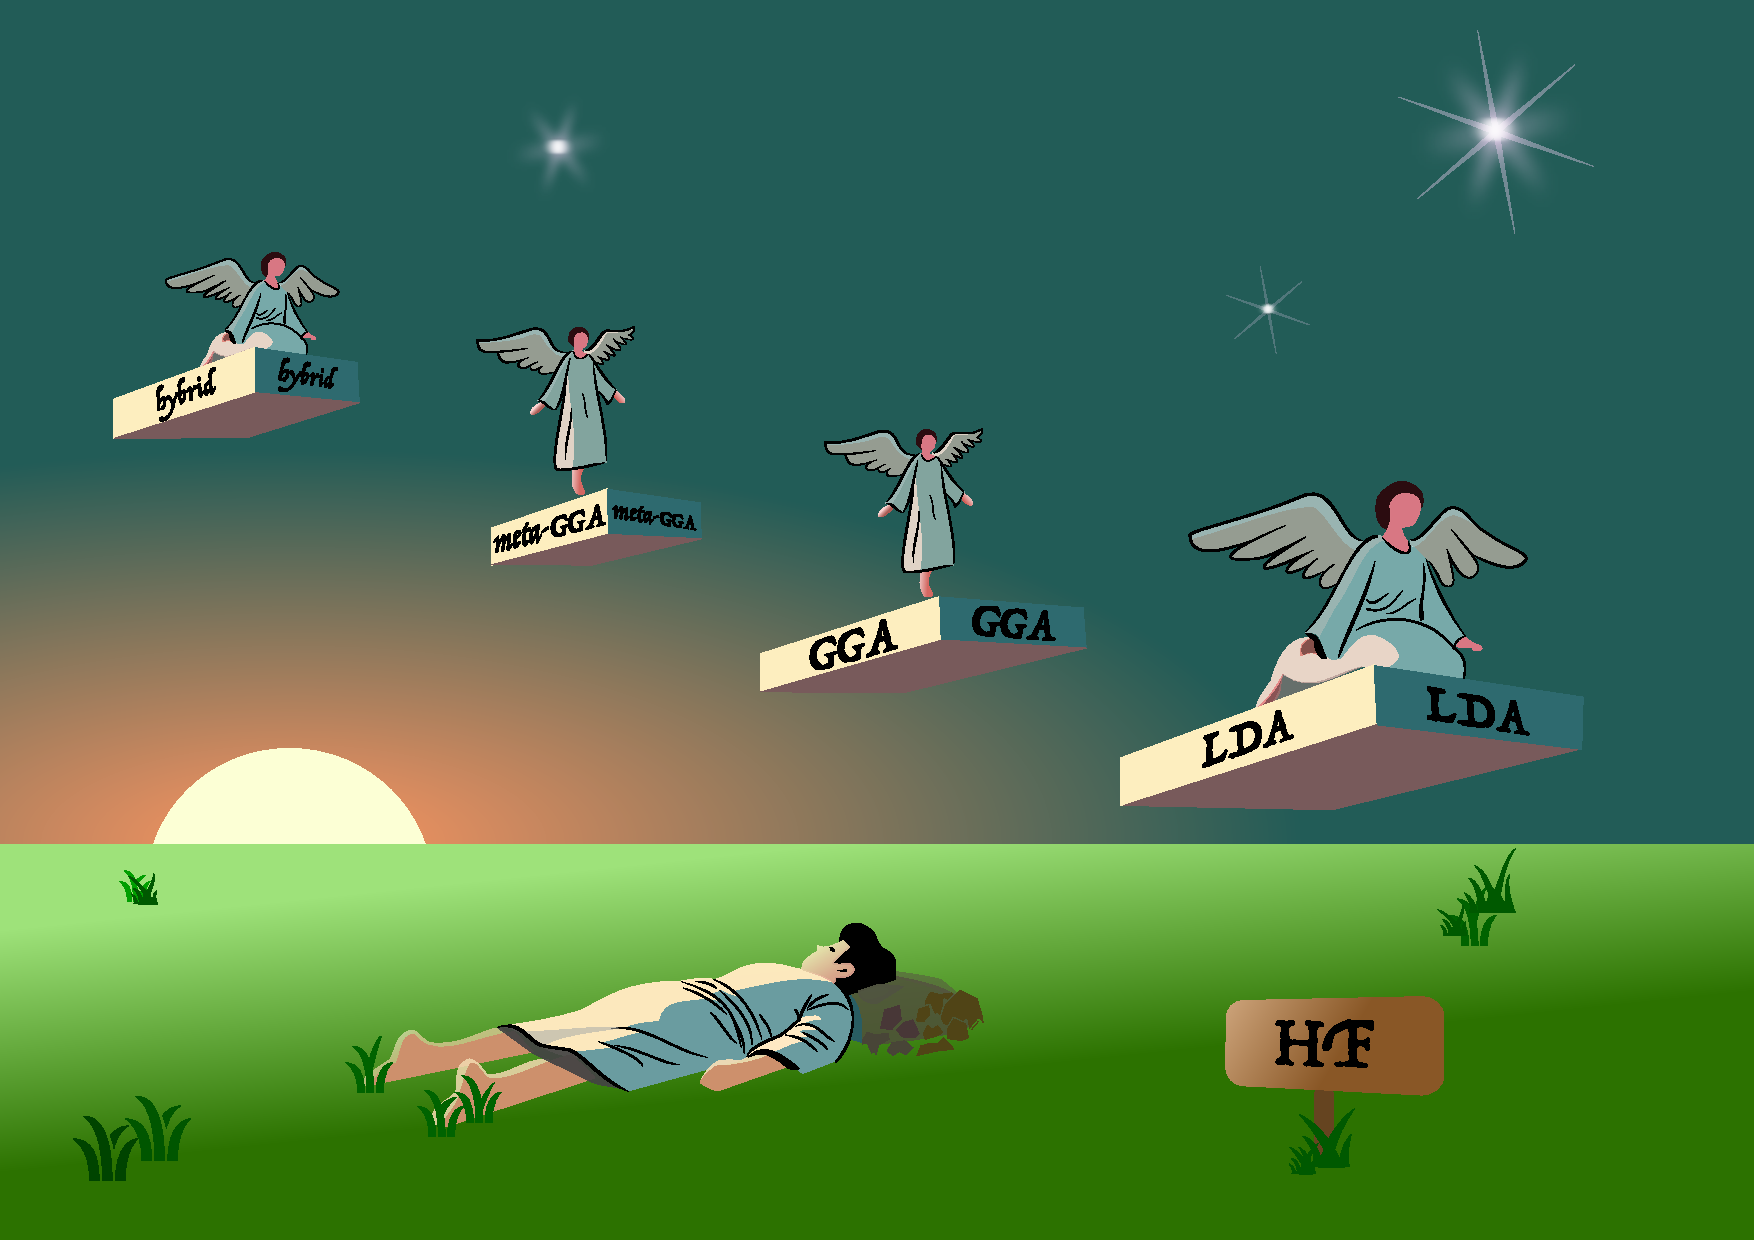
\includegraphics[width=0.8\textwidth]{img/JacobLader.pdf}
  \caption{Jacob's Ladder in \gls{DFT}. Only angels going down, constructing
    the ladder, the rungs are being arrived by the angels.}
\end{figure}


